% Options for packages loaded elsewhere
\PassOptionsToPackage{unicode}{hyperref}
\PassOptionsToPackage{hyphens}{url}
%
\documentclass[
]{book}
\usepackage{amsmath,amssymb}
\usepackage{lmodern}
\usepackage{ifxetex,ifluatex}
\ifnum 0\ifxetex 1\fi\ifluatex 1\fi=0 % if pdftex
  \usepackage[T1]{fontenc}
  \usepackage[utf8]{inputenc}
  \usepackage{textcomp} % provide euro and other symbols
\else % if luatex or xetex
  \usepackage{unicode-math}
  \defaultfontfeatures{Scale=MatchLowercase}
  \defaultfontfeatures[\rmfamily]{Ligatures=TeX,Scale=1}
\fi
% Use upquote if available, for straight quotes in verbatim environments
\IfFileExists{upquote.sty}{\usepackage{upquote}}{}
\IfFileExists{microtype.sty}{% use microtype if available
  \usepackage[]{microtype}
  \UseMicrotypeSet[protrusion]{basicmath} % disable protrusion for tt fonts
}{}
\makeatletter
\@ifundefined{KOMAClassName}{% if non-KOMA class
  \IfFileExists{parskip.sty}{%
    \usepackage{parskip}
  }{% else
    \setlength{\parindent}{0pt}
    \setlength{\parskip}{6pt plus 2pt minus 1pt}}
}{% if KOMA class
  \KOMAoptions{parskip=half}}
\makeatother
\usepackage{xcolor}
\IfFileExists{xurl.sty}{\usepackage{xurl}}{} % add URL line breaks if available
\IfFileExists{bookmark.sty}{\usepackage{bookmark}}{\usepackage{hyperref}}
\hypersetup{
  pdftitle={前端学习笔记},
  pdfauthor={刘卢路},
  hidelinks,
  pdfcreator={LaTeX via pandoc}}
\urlstyle{same} % disable monospaced font for URLs
\usepackage{longtable,booktabs,array}
\usepackage{calc} % for calculating minipage widths
% Correct order of tables after \paragraph or \subparagraph
\usepackage{etoolbox}
\makeatletter
\patchcmd\longtable{\par}{\if@noskipsec\mbox{}\fi\par}{}{}
\makeatother
% Allow footnotes in longtable head/foot
\IfFileExists{footnotehyper.sty}{\usepackage{footnotehyper}}{\usepackage{footnote}}
\makesavenoteenv{longtable}
\usepackage{graphicx}
\makeatletter
\def\maxwidth{\ifdim\Gin@nat@width>\linewidth\linewidth\else\Gin@nat@width\fi}
\def\maxheight{\ifdim\Gin@nat@height>\textheight\textheight\else\Gin@nat@height\fi}
\makeatother
% Scale images if necessary, so that they will not overflow the page
% margins by default, and it is still possible to overwrite the defaults
% using explicit options in \includegraphics[width, height, ...]{}
\setkeys{Gin}{width=\maxwidth,height=\maxheight,keepaspectratio}
% Set default figure placement to htbp
\makeatletter
\def\fps@figure{htbp}
\makeatother
\setlength{\emergencystretch}{3em} % prevent overfull lines
\providecommand{\tightlist}{%
  \setlength{\itemsep}{0pt}\setlength{\parskip}{0pt}}
\setcounter{secnumdepth}{5}
\usepackage{ctex}

%\usepackage{xltxtra} % XeLaTeX的一些额外符号
% 设置中文字体
%\setCJKmainfont[BoldFont={黑体},ItalicFont={楷体}]{新宋体}

% 设置边距
\usepackage{geometry}
\geometry{%
  left=2.0cm, right=2.0cm, top=3.5cm, bottom=2.5cm} 

\usepackage{amsthm,mathrsfs}
\usepackage{booktabs}
\usepackage{longtable}
\makeatletter
\def\thm@space@setup{%
  \thm@preskip=8pt plus 2pt minus 4pt
  \thm@postskip=\thm@preskip
}
\makeatother
\ifluatex
  \usepackage{selnolig}  % disable illegal ligatures
\fi
\usepackage[style=apa,]{biblatex}
\addbibresource{mybib.bib}

\title{前端学习笔记}
\author{刘卢路}
\date{2021年9月28日}

\begin{document}
\maketitle

{
\setcounter{tocdepth}{1}
\tableofcontents
}
\hypertarget{ux524dux8a00}{%
\chapter*{前言}\label{ux524dux8a00}}
\addcontentsline{toc}{chapter}{前言}

勤做笔记不仅可以让自己学的扎实,更重要的是可以让自己少走弯路。有人说:``再次翻开笔记是什么感觉'',我的回答是:``怦然心动的感觉''。或许笔记不一定十全十美,但肯定会让你有种心动💖的感觉。

\hypertarget{part-htmlux57faux7840}{%
\part{HTML基础}\label{part-htmlux57faux7840}}

\hypertarget{ux8ba4ux8bc6web}{%
\chapter{认识Web}\label{ux8ba4ux8bc6web}}

本篇文章主要由五个章节构成,从WEB标准到初识HTML,接着学习HTML常用标签,最后学习表格列表和表单。💪💪开始充电之旅啦\textasciitilde\textasciitilde\textasciitilde{}

\hypertarget{ux7f51ux9875}{%
\section{网页}\label{ux7f51ux9875}}

\textbf{网页}是由文字、图像、音频、视频等元素构成。我们通常看到的网页是以.htm或.html后缀结尾的文件,因此将其俗称为HTML文件,它需要通过浏览器来阅读。

\textbf{网站}是网页的集合。

\textbf{HTML}是超文标记语言(Hyper Text Makeup Language),它是一种用来描述网页的一种语言。
HTML不是编程语言,而是一种标记语言(Makeup language),标记语言是一套标签标记(Makeup tag)。
所谓超文本,有两层含义:

\begin{itemize}
\tightlist
\item
  它可以加入图片、声音、动画、多媒体等内容(超越了文本显著)
\item
  它可以从一个文件跳转到另一个文件,与世界各地主机文件连接(炒鸡连接文本)
\end{itemize}

\textbf{网页的形成}
网页是由网页元素组成的,这些元素是利用html标签描述出来,然后通过浏览器解析出来显示给用户。
前端人员开发代码→浏览器显示代码(解析、渲染)→生成Web页面

\hypertarget{ux6d4fux89c8ux5668}{%
\section{浏览器}\label{ux6d4fux89c8ux5668}}

\textbf{浏览器}是显示、运行网页的平台。IE、火狐(Firefox)、谷歌(Chrome)、Safari和欧鹏(Opera)被称为五大浏览器。

\textbf{浏览器内核}排版引擎、解释引擎、渲染引擎。负责读取网页内容,整理讯息,计算网页的显示方式并显示页面。

\begin{table}

\caption{\label{tab:unnamed-chunk-1}浏览器内核}
\centering
\begin{tabular}[t]{lll}
\toprule
浏览器 & 内核 & 备注\\
\midrule
IE & Trident & IE、猎豹安全、360极速浏览器、百度浏览器\\
Firefox & Gecko & 可惜这几年已经没落了,打开速度慢、升级频繁、猪一样的队友flash、神一样的对手chrome。\\
Safari & Webkit & 现在很多人错误地把 webkit 叫做 chrome内核(即使 chrome内核已经是 blink 了)。苹果感觉像被别人抢了媳妇,都哭晕在厕所里面了。\\
Chrome & Chromium/Blink & 在 Chromium 项目中研发 Blink 渲染引擎(即浏览器核心),内置于 Chrome 浏览器之中。Blink 其实是 WebKit 的分支。大部分国产浏览器最新版都采用Blink内核。二次开发\\
Opera & Blink & 现在跟随chrome用blink内核。\\
\bottomrule
\end{tabular}
\end{table}

\hypertarget{webux6807ux51c6}{%
\section{Web标准}\label{webux6807ux51c6}}

Web标准是由W3C组织和其他标准化组织制定的一系列标准的集合。W3C(万维网联盟)是国际最著名的标准化组织。

\hypertarget{ux4e3aux4ec0ux4e48ux9700ux8981webux6807ux51c6}{%
\subsection{为什么需要Web标准}\label{ux4e3aux4ec0ux4e48ux9700ux8981webux6807ux51c6}}

浏览器不同,它们显示页面或者排版就有些许差异。
遵循Web标准除了可以让不同开发人员写出的页面更标准,更统一外,还有以下优点:👇

\begin{itemize}
\tightlist
\item
  易于维护:只需更改CSS文件,就可以改变整站的样式
\item
  页面响应快:HTML文档体积变小,响应时间短
\item
  可访问性:语义化的HTML(结构和表现相分离的HTML)编写的网页文件,更容易被屏幕阅读器识别
\item
  设备兼容性:不同的样式表可以让网页在不同的设备上呈现不同的样式
\item
  搜索引擎:语义化的HTML能更容易被搜索引擎解析,提升排名
\end{itemize}

\hypertarget{webux6807ux51c6ux6784ux6210}{%
\subsection{Web标准构成}\label{webux6807ux51c6ux6784ux6210}}

主要包括结构标准(Structure),表现标准(Presentation)和行为标准(Behavior)。

\begin{itemize}
\tightlist
\item
  结构标准用于对网页元素进行整理和分类,现阶段主要学的是HTML
\item
  表现标准用于设置网页元素的版式、颜色、大小等外观属性,主要指的是CSS
\item
  行为标准用于对网页模型的定义及交互的编写,现阶段主要学的是JavaScript
\end{itemize}

\begin{table}

\caption{\label{tab:unnamed-chunk-2}Web标准}
\centering
\begin{tabular}[t]{ll}
\toprule
标准 & 说明\\
\midrule
结构标准 & 用于对网页元素进行整理和分类,现阶段主要学的是HTML\\
表现标准 & 用于设置网页元素的版式、颜色、大小等外观属性,主要指的是CSS\\
行为标准 & 用于对网页模型的定义及交互的编写,现阶段主要学的是JavaScript\\
\bottomrule
\end{tabular}
\end{table}

Web标准提出的最佳体验方案:\textbf{结构、样式、行为相分离}。简单理解:结构写到HTML文件中、表现写到CSS文件中、行为写到JavaScript中。

\begin{figure}

{\centering 
\includegraphics{fig/1-1} 

}

\caption{Web标准}\label{fig:unnamed-chunk-3}
\end{figure}

\hypertarget{htmlux521dux8bc6}{%
\chapter{HTML初识}\label{htmlux521dux8bc6}}

\hypertarget{ux57faux672cux8bedux6cd5ux89c4ux8303}{%
\section{基本语法规范}\label{ux57faux672cux8bedux6cd5ux89c4ux8303}}

\hypertarget{ux57faux672cux8bedux6cd5ux6982ux8ff0}{%
\subsection{基本语法概述}\label{ux57faux672cux8bedux6cd5ux6982ux8ff0}}

HTML标签是由尖括号包围的关键词,例如\texttt{\textless{}html\textgreater{}}。

HTML标签通常是成对出现的,例如\texttt{\textless{}html\textgreater{}}和\texttt{\textless{}/html\textgreater{}},我们称为双标签。标签对中的第一个标签是开始标签,第二个标签是结束标签。

有些特殊标签必须是单个标签(极少情况),例如\texttt{\textless{}br\ /\textgreater{}},我们称为单标签。

\hypertarget{ux6807ux7b7eux5173ux7cfb}{%
\subsection{标签关系}\label{ux6807ux7b7eux5173ux7cfb}}

双标签关系可以分为两类:包含关系和并列关系。

包含关系,又被称为父子关系。
eg:title标签包含于head标签中。

\begin{verbatim}
<head>
    <title></title>
</head>
\end{verbatim}

并列关系,又被称为兄弟关系。
eg:title标签和head标签并列。

\begin{verbatim}
<head></head>
<body></body>
\end{verbatim}

\hypertarget{ux57faux672cux7ed3ux6784ux6807ux7b7e}{%
\section{基本结构标签}\label{ux57faux672cux7ed3ux6784ux6807ux7b7e}}

每个网页都会有一个基本的结构标签(也被称为骨架标签),页面内容也是在这些基本标签上书写。HTML页面也称为HTML文档。

\begin{verbatim}
<html>
    <head>     
        <title>第一个页面</title> 
    </head>
    <body>
         键盘敲烂,工资过万
    </body>
</html>
\end{verbatim}

HTML文档的后缀名必须是.htm或.html,浏览器的作用是读取HTML文档,并以网页形式显示他们。此时,用浏览器打开这个网页,我们就可以预览我们写的HTML文件了。

\begin{table}

\caption{\label{tab:unnamed-chunk-1}基本结构标签}
\centering
\begin{tabular}[t]{lll}
\toprule
标题名 & 定义 & 说明\\
\midrule
`<heml></html>` & HTML标签 & 页面中最大的标签,我们称为根标签\\
`<head></head>` & 文档头部 & 注意head标签中我们必须要设置的标签是tittle\\
`<title></title>` & 文档标题 & 让页面拥有一个属于自己的网页标题\\
`<body></body>` & 文档主体 & 元素包含文档的所有内容,页面内容基本都是放到body里面\\
\bottomrule
\end{tabular}
\end{table}

\begin{figure}

{\centering 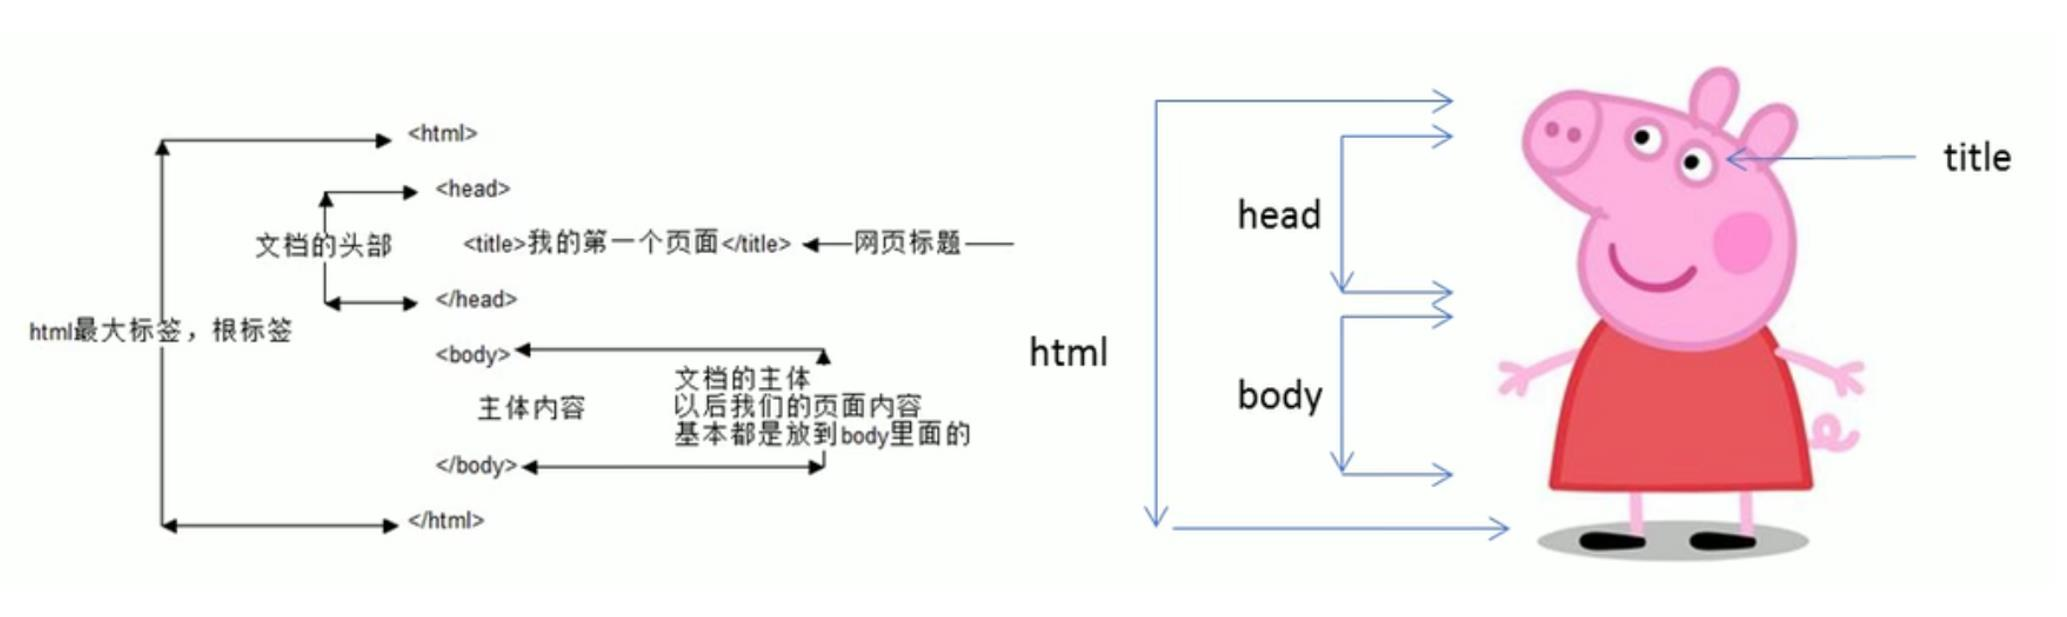
\includegraphics{fig/1-2} 

}

\caption{HTML骨架标签}\label{fig:unnamed-chunk-2}
\end{figure}

\hypertarget{ux7f51ux9875ux5f00ux53d1ux5de5ux5177}{%
\chapter{网页开发工具}\label{ux7f51ux9875ux5f00ux53d1ux5de5ux5177}}

\hypertarget{ux914dux7f6evscode}{%
\section{配置VSCode}\label{ux914dux7f6evscode}}

下载并安装\href{https://code.visualstudio.com/download}{Visual Studio Code软件}

新建文件(快捷键\texttt{Ctrl}+\texttt{N}),然后保存(快捷键\texttt{Ctrl}+\texttt{S})后缀名为.html的文件,在第一行代码中输入\texttt{!},再按\texttt{Tab}键,即可自动生成HTML的骨架文件。安装插件(Open in Browser)后可在浏览器中预览,单击鼠标右键,在弹出窗口中点击\texttt{Open\ in\ Default\ Browser}。\\
接下来介绍一下如何安装插件。

\begin{figure}

{\centering 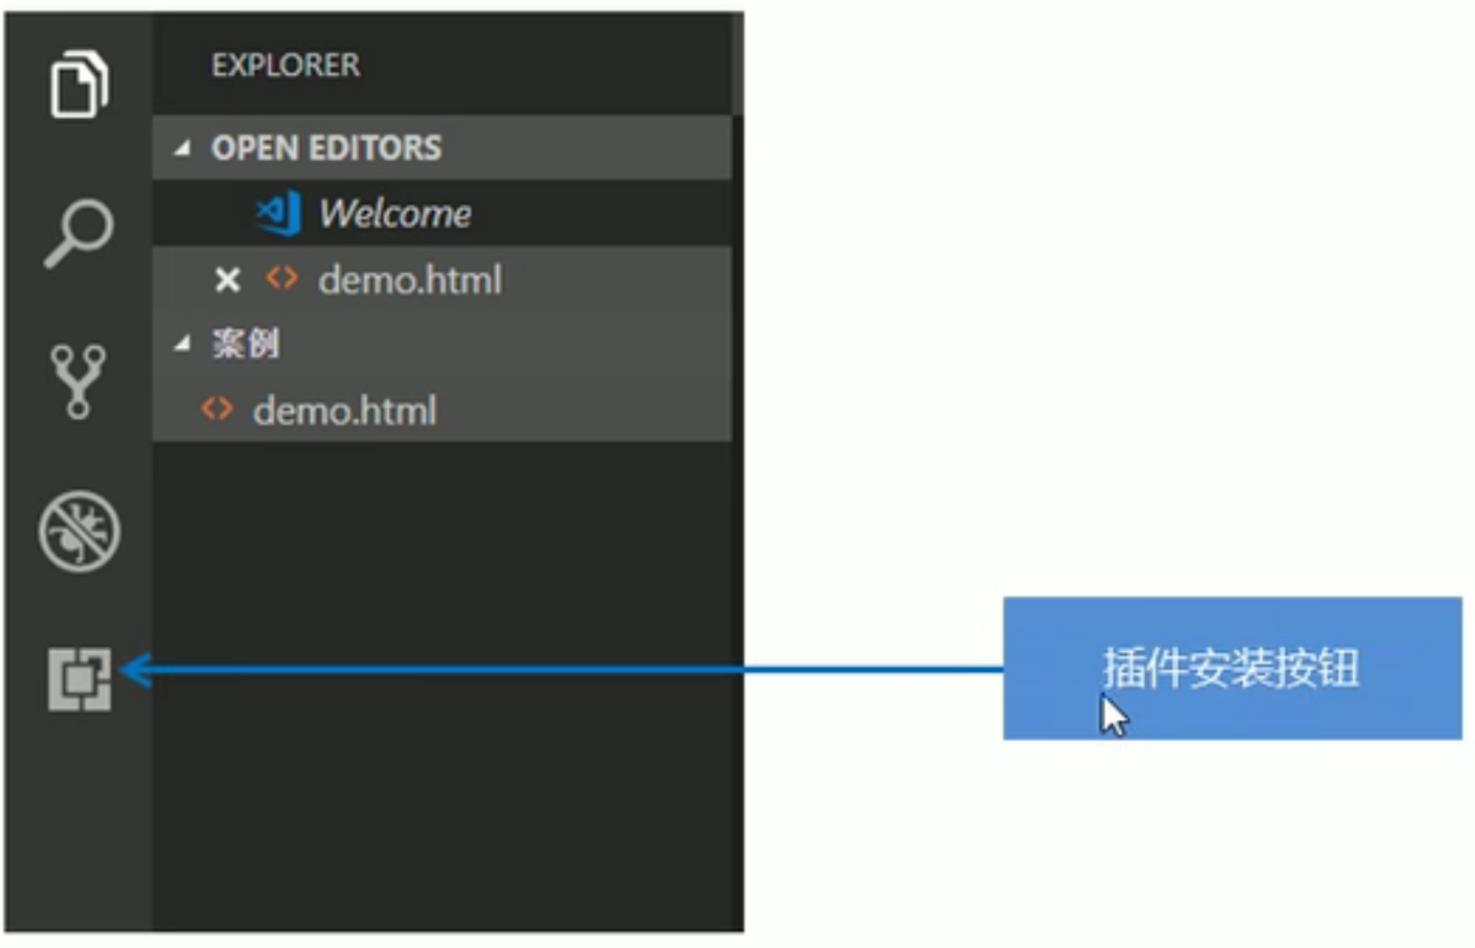
\includegraphics[width=0.5\linewidth]{fig/1-4} 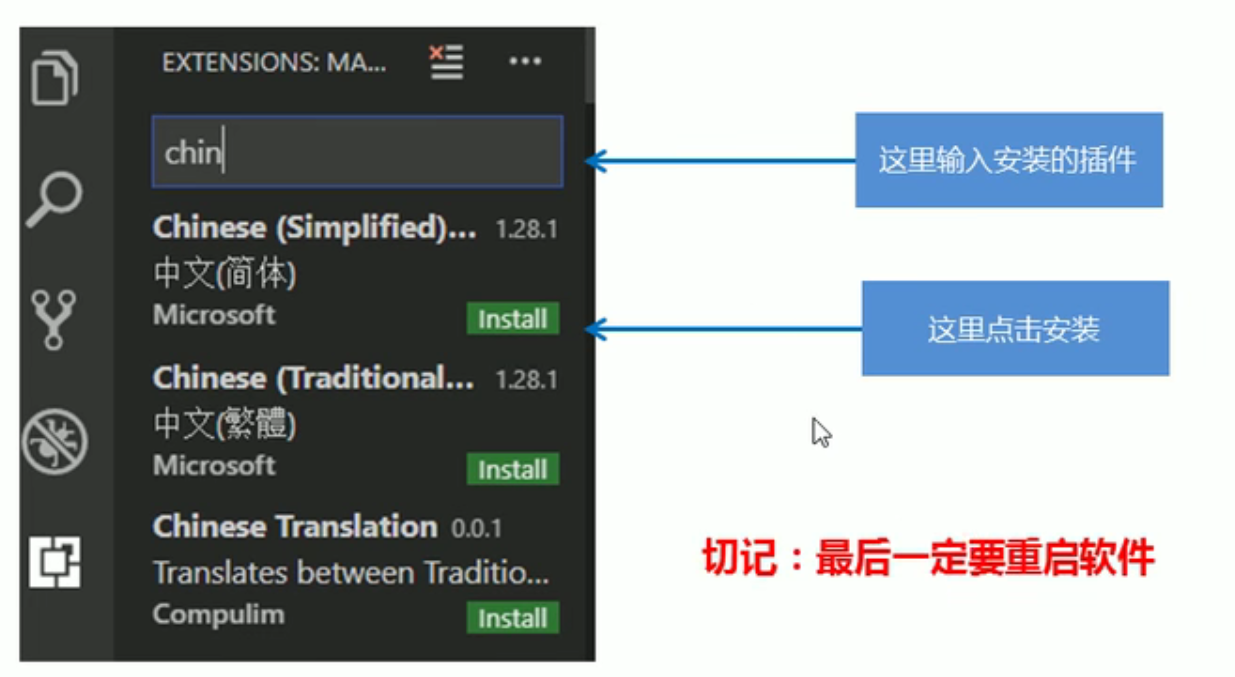
\includegraphics[width=0.5\linewidth]{fig/1-5} 

}

\caption{安装插件}\label{fig:unnamed-chunk-1}
\end{figure}

一些常用的插件:

\begin{table}

\caption{\label{tab:unnamed-chunk-2}基本结构标签}
\centering
\begin{tabular}[t]{ll}
\toprule
插件 & 作用\\
\midrule
Chinese (Simplified) Language Pack of VS Code & 中文(简体)语言包\\
Open in Browser & 右键选择浏览器打开HTML文件\\
JS-CSS-HTML Formatter & 每次保存,都会自动格式化JS CSS和HTML代码\\
Auto Rename Tag & 自动重命名配对的HTML/XML标签\\
CSS peek & 追踪至样式\\
\bottomrule
\end{tabular}
\end{table}

\hypertarget{vscodeux5de5ux5177ux751fux6210ux9aa8ux67b6ux6807ux7b7eux65b0ux589eux4ee3ux7801}{%
\section{VSCode工具生成骨架标签新增代码}\label{vscodeux5de5ux5177ux751fux6210ux9aa8ux67b6ux6807ux7b7eux65b0ux589eux4ee3ux7801}}

\hypertarget{ux6587ux6863ux7c7bux578bdoctype}{%
\subsection{\texorpdfstring{文档类型\texttt{\textless{}!DOCTYPE\textgreater{}}}{文档类型\textless!DOCTYPE\textgreater{}}}\label{ux6587ux6863ux7c7bux578bdoctype}}

\texttt{\textless{}!DOCTYPE\textgreater{}}是文档类型(Document type)声明,作用是告诉浏览器使用哪种HTML版本来显示网页。

\begin{verbatim}
<!DOCTYPE html>
\end{verbatim}

这句代码的意思是:当前页面采取的是HTML5版本来显示网页。注意\texttt{\textless{}!DOCTYPE\textgreater{}}声明位于文档中的首行,处于\texttt{\textless{}html\textgreater{}}标签之前,\texttt{\textless{}!DOCTYPE\textgreater{}}不是一个HTML标签,它就是文档类型声明标签。
\#\#\# 页面语言\texttt{lang}

\texttt{lang}用来定义当前文档显示的语言(language)。\texttt{en}定义语言为英语,\texttt{zh-CN}定义语言为中文。其实对于文档显示来说,定义成\texttt{en}的文档也可以显示中文,定义成\texttt{zh-CN}的文档也可以显示英文这个属性对浏览器和搜索引擎(百度.谷歌等)还是有作用的。

\hypertarget{ux5b57ux7b26ux96c6charset}{%
\subsection{\texorpdfstring{字符集\texttt{charset}}{字符集charset}}\label{ux5b57ux7b26ux96c6charset}}

字符集(Character set)是多个字符的集合。以便计算机能够识别和存储各种文字。在\texttt{\textless{}head\textgreater{}}标签内,可以通过\texttt{\textless{}meta\textgreater{}}标签的\texttt{charset}属性来规定HTML文档应该使用哪种字符编码。

\begin{verbatim}
<meta charset=" UTF-8"/>
\end{verbatim}

charset常用的值:GB2312、BlG5、GBK和UTF-8,其中\textbf{UTF-}8也被称为\textbf{万国码},基本包含了全世界所有国家需要用到的字符。\\
注意∶上面语法是必须要写的代码,否则可能引起乱码的情况。一般情况下,统一使用``UTF-8''编码,尽量统一写成标准的``UTF-8'',不要写成``utf8''或``UTF8''。

\hypertarget{htmlux5e38ux7528ux6807ux7b7e}{%
\chapter{HTML常用标签}\label{htmlux5e38ux7528ux6807ux7b7e}}

\hypertarget{ux8bedux4e49ux6807ux7b7e}{%
\section{语义标签}\label{ux8bedux4e49ux6807ux7b7e}}

学习标签是有技巧的,重点是记住每个标签的语义。简单理解就是指\textbf{标签的含义},即这个标签是用来干嘛的。\textbf{根据标签的语义,在合适的地方给一个最为合理的标签,可以让页面结构更清晰。}

\begin{figure}

{\centering 
\includegraphics{fig/1-6} 

}

\caption{语义标签}\label{fig:unnamed-chunk-1}
\end{figure}

\hypertarget{ux6807ux9898ux6807ux7b7e}{%
\section{标题标签}\label{ux6807ux9898ux6807ux7b7e}}

为了使网页更具有语义化,我们经常会在页面中用到标题标签。HTML提供了6个等级的网页标题,即\texttt{\textless{}h1\textgreater{}} - \texttt{\textless{}h6\textgreater{}}。

\begin{verbatim}
<h1>我是一级标题</h1>
\end{verbatim}

h单词head 的缩写,意为头部、标题。
\textbf{标签语义}:作为标题使用,并且依据重要性递减。\\
特点:

\begin{itemize}
\tightlist
\item
  加了标题的文字会变的加粗,字号也会依次变大。
\item
  一个标题独占一行。
\end{itemize}

\begin{verbatim}
<h1>标题一共六级选,</h1>
<h2>文字加粗一行显。</h2>
<h3>由大到小依次减,</h3>
<h4>从重到轻随之变。</h4>
<h5>语法规范书写后,</h5>
<h6>具体效果刷新见。</h6>
\end{verbatim}

\hypertarget{ux6bb5ux843dux6807ux7b7e}{%
\section{段落标签}\label{ux6bb5ux843dux6807ux7b7e}}

在网页中,要把文字有条理地显示出来,就需要将这些文字分段显示。在HTML标签中,\texttt{\textless{}p\textgreater{}}标签用于定义段落,它可以将整个网页分为若干个段落。

\begin{verbatim}
<p>我是一个段落标签</p>
\end{verbatim}

p是单词paragraph的缩写,意为段落。\textbf{标签语义}:可以把HTML文档分割为若干段落。

特点∶

\begin{itemize}
\tightlist
\item
  文本在一个段落中会根据浏览器窗口的大小自动换行。
\item
  段落和段落之间保有空隙。
\end{itemize}

\hypertarget{ux6362ux884cux6807ux7b7e}{%
\section{换行标签}\label{ux6362ux884cux6807ux7b7e}}

在HTML中,一个段落中的文字会从左到右依次排列,直到浏览器窗口的右端,然后才自动换行。如果希望某段文本强制换行显示,就需要使用换行标签\texttt{\textless{}br\ /\textgreater{}}。

\begin{verbatim}
<br />
\end{verbatim}

br是单词break的缩写,意为打断、换行。标签语义∶强制换行。

特点︰

\begin{itemize}
\tightlist
\item
  \texttt{\textless{}br\ /\textgreater{}}是个单标签。
\item
  \texttt{\textless{}br\ /\textgreater{}}标签只是简单地开始新的一行,跟段落不一样,段落之间会插入一些垂直的间距。
\end{itemize}

\hypertarget{ux6587ux672cux683cux5f0fux5316ux6807ux7b7e}{%
\section{文本格式化标签}\label{ux6587ux672cux683cux5f0fux5316ux6807ux7b7e}}

在网页中,有时需要为文字设置粗体、斜体或下划线等效果,这时就需要用到HTML中的文本格式化标签,使文字以特殊的方式显示。
标签语义:突出重要性,比普通文字更重要.

\begin{table}

\caption{\label{tab:unnamed-chunk-2}文本格式化标签}
\centering
\begin{tabular}[t]{lllll}
\toprule
语义 & 标签 & 单词 & 实例 & 说明\\
\midrule
加粗 & `<strong></strong>`或者`<b></b>` & strong & <strong>强调</strong> & 更推荐使用`<strong>`标签加粗语义更强烈\\
倾斜 & `<em></em>`或者`<i></i>` & emphasize & <em>斜体</em> & 更推荐使用`<em>`标签加粗语义更强烈\\
删除线 & `<del></del>`或者`<s></s>` & delete & <del>删除线</del> & 更推荐使用`<del>`标签加粗语义更强烈\\
下划线 & `<ins></ins>`或者`<u></u>` & inserted & <ins>下划线</ins> & 更推荐使用`<ins>`标签加粗语义更强烈\\
\bottomrule
\end{tabular}
\end{table}

\hypertarget{ux6848ux4f8bux5b66ux4e60}{%
\section{案例学习}\label{ux6848ux4f8bux5b66ux4e60}}

\begin{figure}

{\centering 
\includegraphics{fig/1-7} 

}

\caption{案例学习}\label{fig:unnamed-chunk-3}
\end{figure}

\begin{verbatim}
<!DOCTYPE html>
<html lang="en">
<head>
    <meta charset="UTF-8">
    <meta http-equiv="X-UA-Compatible" content="IE=edge">
    <meta name="viewport" content="width=device-width, initial-scale=1.0">
    <title>Document</title>
</head>
<body>
    <h1>水花61分伊戈达拉制胜抢断西决勇士再胜开拓者总分2-0</h1>
    <h4>数据统计:水花兄弟合砍61分</h4>
    <p>
        库里22投11中,三分14投4中,罚球11罚全中得到37分8篮板8助攻,职业生涯季后赛得分30+次数来到35次
        超过哈登排名现役第3位,仅次于詹姆斯和杜兰特。
    </p>   
    <p>
        汤普森22投8中,三分8投4中得到24分3篮板2助攻,德拉蒙德-格林得到16分10篮板7助攻5盖帽,凯文-鲁尼得到14分7篮板2助攻,今天勇士有7名替补出场。
    </p>
    <h4>兄弟对决升级:小库里给哥哥造成压力</h4>
    <p>
        库里兄弟是NBA历史上第一对在分区决赛相遇的兄弟。在西决第1场中,小库里没有给哥哥造成压力,他出场19分钟,7投1中只得到3分3篮板2助攻,在场期间输掉10分。
    </p>
    <p>
        但在西决第2场中,小库里攻防两端都打出杰出的表现,全场送出4次抢断,包括直接抢断自己的哥哥库里,在防守端给库里造成了极大的困扰。
    </p>
    <p>
        作者: pink老师<br />2019-8-8
    </p>
</body>
</html>
\end{verbatim}

\hypertarget{part-ux9644ux5f55}{%
\part{附录}\label{part-ux9644ux5f55}}

\hypertarget{vscodeux5e38ux7528ux64cdux4f5c}{%
\chapter{Vscode常用操作}\label{vscodeux5e38ux7528ux64cdux4f5c}}

快捷键\\
- 创建文件:\texttt{Ctrl+}N\texttt{-\ 保存文件:}Ctrl+\texttt{S}
- 放大页面:\texttt{Ctrl}+\texttt{+}
- 缩小页面:\texttt{Ctrl}+\texttt{-}
- 预览页面:\texttt{Alt}+\texttt{B},或单击鼠标右键,在弹出窗口中点击\texttt{Open\ in\ Default\ Browser}
- 自动换行:\texttt{Alt}+\texttt{Z},或在\texttt{查看}中选择\texttt{自动换行}

\hypertarget{section}{%
\chapter{4}\label{section}}

\printbibliography

\end{document}
